% !TEX root = ../zenkoku.tex
\section{結果}
アンケートは部の開発者全員である9人全員から回答を得た.

集計方法としては熟練した開発者を1人想定し,この開発者への依存度が高いようなシステムを洗い出すことにした.
理解度は値が高いほど理解が深いものとし,`熟練者の理解度 - 熟練者を除いた回答者の理解度平均` によって求めた数値を熟練者への依存度の高さとする.
結果を\ri{img:rikai}に示す.

属人性の高さとしてはシステムAやシステムBのフロントエンド領域などにおいて熟練者への依存度の高さが圧倒的だが,システムGのように差が0.4ポイントしか見られないようなものもある.
またシステムKやシステムHのバックエンド領域など熟練者,平均ともに理解度の低いものも見受けられ,これは開発組織内で誰も詳細を知らないシステムとなっていると考えられる.

この結果を開発組織内に対し討論する機会を設けたところ以下のような意見が出た.

% ここの書き方考え中
- 熟練者への依存度を下げたい という思いはあるが何から始めたらいいかわからない状況がある. good First issue とかを用意してはどうか
- hoge

\begin{figure}
	\centering
	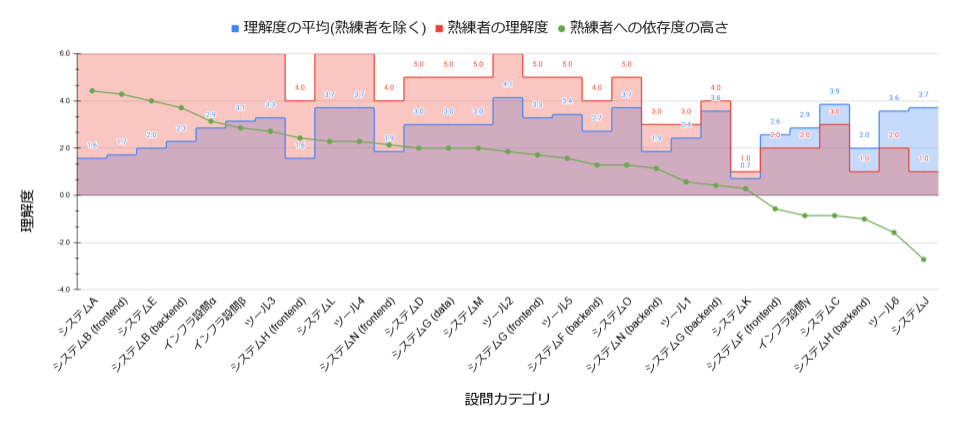
\includegraphics[keepaspectratio,width=0.9\linewidth]{img/rikai.png}
	\caption{理解度の平均と熟練者への依存度の高さ}
	\label{img:rikai}
\end{figure}
